%!TEX root = ../main.tex

\chapter{Confocal Setup}	\label{ch::confocal_setup}
\chaptermark{Confocal Setup}

	The key measurements of this thesis are fluorescence measurements of \sivs in nanodiamonds.
	For this aim, a home-built confocal setup is used, which is described in this chapter.

	The confocal setup serves to perform a series of measurements on \fl: scanning the sample to find \sivs, recording luminescence spectra of the aforementioned, determine the saturation count rate \todo{saturation already introduced?}, and determine whether the emitter in question is a single emitter by performing photon autocorrelation measurements.
	The key components for these measurements are 

	\begin{itemize}
		\item The confocal unit which serves to excite the emitters and collect the \fl and move the sample while scanning.
		\item A grating spectrometer to investigate the spectral properties of the emitters. This is crucial to distinguish between \sivs, other \ccs and "dirt".
		\item A \keyword{\HBT} (\hbt) setup to investigate the single photon character. It is built up of two avalanche photo diodes (APDs) which also serve to scan the sample in order to find emitters on the sample surface; and to perform saturation measurements.
	\end{itemize}

	\begin{figure}[t] %fig::confocal_setup
		\begin{minipage}{.5\textwidth}
			\centering
			\testbox{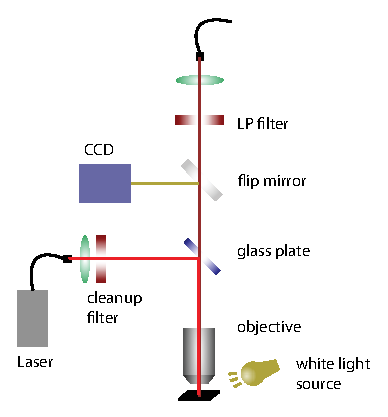
\includegraphics{./pics/confocal_setup_small.eps}}
			\caption{Confocal setup}
			\label{fig::confocal_setup}
		\end{minipage}
		\hfill
		\begin{minipage}{.5\textwidth}
			\centering
			\testbox{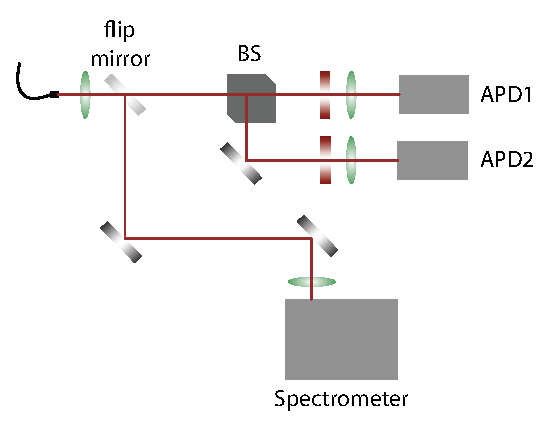
\includegraphics{./pics/hbt_spectrometer.eps}}
			\caption{HBT, spectrometer}
			\label{fig::hbt_spectrometer}
		\end{minipage}
	\end{figure}	


	\section[Confocal Unit]{Confocal Unit}

		\autoref{fig::confocal_setup} depicts a sketch of the confocal setup. 
		Except for the laser and the sample stage, the whole setup is fixed to a vertical breadboard. 
		This design allows for easy scanning and exchanging of the samples, without the need of gluing them to a vertical stage.
		The friction between the sample and the aluminum surface of the stage is sufficient that the sample does not move during scanning.
		If it is important that the sample has a a defined orientation, it is put inside of an aluminum angle.
		The stage is powered with two stepper motors (\todo{type}) in the horizontal x and y directions.
		The objective is fixed to another stage which in turn is fixed to the vertical breadboard.
		In this way, the vertical z direction is implemented for focusing the laser light on the sample.
		Therefore, a three-axis scanning of the sample is implemented.

		The bright red color at the left-hand side of the sketch represents the excitation beam path.
		The sample is excited with a continuous wave diode laser (Sch\"after-Kirchhoff, 58FCM) which emits at a \wl of \SI{660}{\nano\meter}.
		The outlet of the light is through a pigtail fiber, the light is outcoupled and collimated exploiting an aspheric lens.
		To suppress sideband emission from the laser, a bandpass filter with a window of  \SI{10}{\nm} around a center of \SI{660}{\nm} is used.
		The excitation beam then hits a glass plate (fabricator Halle Germany \todo{thickness}) to be guided through a microscope objective and focused on the sample.
		The microscope objective is of the type Olympus, LMPlanFLN 100x and has a numerical aperture of 0.8.
		As the luminescence light from the emitter is in the same focus as the excitation laser light, it is effectively collected by the objective (hence "confocal setup").

		The collected light then follows the detection beam path depicted in a dark red color in \autoref{fig::confocal_setup}.
		Both the excitation light reflected from the sample surface and the \fl pass through the glass plate.
		In the usual useage, the flip mirror just after the beamsplitter is lowered, allowing the light coming from the sample to move on towards a single mode fiber. 
		In front of the \smf there is a longpass filter of a cutoff \wl of \SI{710}{\nm} or \SI{720}{\nm} to filter out the residual excitation light and also ambient light.
		The \fl is fed into a single-mode fiber (Thorlabs SM600) with an aspheric lens.
		The single-mode fiber serves two purpuses: First, to connect the confocal microscope with the \hbt setup and the spectrometer.
		Second, its about \SI{4.3}{\micro\meter} diameter serves as a pinhole to ensure optimal resolution. 
		In the direction of the optical axis the resolution amounts to \todo{value}, in the plane of the sample it is \todo{value}.
		\todo{short discussion if resolution is enough}

		According to the experimental necessities, instead of the mentioned glass plate a dichroic mirror (\todo{which?}) can be employed.
		A dichroic mirror spectrally separates the incident light by transmitting and reflecting it as a function of the wavelength. 
		Hence, excitation light is separated from \fl.
		The glass plate features a high transmission of 90\%\todo{check number} and therefore a high collection efficiency of \fl, whereas the dichroic mirror allows for a higher excitation intensity using the same excitation laser. 
		However, a high excitation intensity may cause permanent fluorescence intermittence of the \sivs (for further detail, refer to \todo{insert chapter}).
		In general, if a high excitation is necessary, for instance for saturation measurements \todo{saturation already introduced?}, the dichroic mirror is used; otherwise, the glass plate is used to collect as much \fl as possible.

	\section[Sample Surface]{Optical Imaging of The Sample Surface}

		Another feature of the setup is that it is possible to have a look at the sample surface before starting the fluorescence measurements.
		For this purpose, the sample is illuminated with white light from a halogen lamp and the flip mirror after the glass plate is brought into an upright position to guide the light onto a CCD camera (\todo{specs}).
		The scattered light from the sample surface is collected by the objective and the surface is shown on the CCD image.
		Nanodiamonds and other features on the substrate are visible, the resolution of this setup is limited by \todo{optical diffraction, shadows}.
		However, it suffices to find the markers of a dimension of \SI{10}{\micro\meter} which were milled into some substrates and to recognize characteristic patterns of the coated \nds.

	\section[Spectrometer]{Spectrometer}

		\autoref{fig::hbt_spectrometer} displays the detector part of the setup.
		The \fl in the fiber coming from the confocal unit is outcoupled with an aspheric lens. 
		A flip mirror is employed to direct the light either to a grating spectrometer or the \hbt setup.

		As mentioned before, the \fl from the \sivs is investigated with the grating spectrometer to evaluate the source of the \fl by comparing the measured spectrum to typical spectra from known sources.
		The spectrometer is a Princeton Instruments Acton2500i \todo{?} spectrometer.
		The incident beam passes through an entrance slit, is then scattered on the grating where the light is spectrally divided and finally hits a detector, imaging the entrance slit on the detector surface.
		The employed detector is a CCD camera ()\todo{type} which is cooled with liquid nitrogen for noise reduction.
		It enables detection of light up to a \wl of \SI{1000}{nm}.
		The spectrometer features three gratings: \SI[per-mode=symbol]{600}{\lines\per\mm}, \SI[per-mode=symbol]{1200}{\lines\per\mm}, and \SI[per-mode=symbol]{1800}{\lines\per\mm}.
		With a step-and-glue function of the spectrometer software (WinSpec) it is possible, to record several spectra over a wide \wl range which are then stiched together.
		It is therefore possible to combine a larger \wl range with a higher resolution.
		For most measurements the grating with \SI[per-mode=symbol]{600}{\lines\per\mm} was used. 
		The resolution of the spectrometer using the \SI{600}{\lines\per\mm} is \verify{xx} as stated by the manufacturer.
		This resolution suffices for most of the measurements mentioned in this work.

	\section[HBT]{\HBT Setup}

		An \majorkeyword{\HBT setup} serves to record the \keyword{photon autocorrelation function} (\keyword{\gt function}) of an emitter.
		In the photon number representation, it is defined as follows:
		\[
		\gtz = \frac{ \mean{ N(t) N(t+\tau) } }{\mean{N(t)}^2}.
		\]
		Here, $N(t)$ denotes the photon at a certain time $t$, $N(t+\tau)$ denotes the photon at a time interval $\tau$ later than $t$.
		The angular brackets $\mean{}$ denote the temporal averaging.
		In this work, the \gtf is used to make statements about whether the emitter emits single photon and is therefore one single emitter.
		The physical explanation is \todo{fox nachlesen} that if the emitter is a single emitter and emits at a time $t$, the next time any photon is recorded is at time $t+\tau$.
		For a time interval close to zero, the value of the \gtf must ideally approach zero or at least be smaller than \num{0.5} if only a single emitter is present:
		The denominator is zero, because $N(t + \tau) (\tau = 0)=0$ due to only one photon, namely $N(t)$ being present.
		If two photons are emitted at the same time (time delay zero), the \gtf yields $\gtz=0.5$. 
		(For a detailed explanation of the \gtf read \cite{fox})

		The principle of the \hbt setup is to evaluate the time delay between two consecutive photons. 
		The photons are detected with \apds of the type PicoQuant $\tau${}-SPAD 100 \todo{100?}.
		These \apds have a nominal detection efficiency of up to 70\% at the optimal wavelength of about \SI{670}{\nm}, a dark count rate of under \SI{100}{\cps}, and a dead time to avoid afterpulsing of about \SI{70}{\ns}.
		In the ideal case, one \APD would be enough to measure the time delay between two consecutive photons. 
		However, the second of two consecutive photons could hit the detector during its dead time.
		To circumvent this problem, two \APDs are employed and the detection beam is split with a non-polarizing 50:50 beamsplitter cube (\todo{type}).
		Each beam then passes through a bandpass filter and is focused on the \apd with a lens \todo{welche?}.
		The bandpass filters serve two \verify{reasons}:
		First, they limit optical crosstalk between the \apds. 
		The process of detection of an \apd produces light due to recombination of charge carriers. 
		Crosstalk between two \apds occurs, if one of the photons produced by one \apd escapes and is detected in the other one \cite{Younger2009}.  
		Secondly the bandpass filters serve to reduce \bkg during the \gt measurement process or to spectrally divide emission from several emitters.
		Therefore, it is possible to find single emitters, which are not spatially seperated enough to be seperated with the spatial resolution of the setup, but can be spectrally seperated if their \ZPLs are apart enough that respective bandpass filters can be used to only investigate light from one \ZPL.


		timing jitter, ttl pulses, time tagging module, algorithmus




